% ============================================================
% Figure 5: QualityGate Decision Flow
% ============================================================
\documentclass[border=5pt]{standalone}
\usepackage[T1]{fontenc}
\usepackage{tikz}
\usetikzlibrary{arrows.meta, positioning, shapes.geometric}

\definecolor{cb1}{RGB}{0,101,189}
\definecolor{cb2}{RGB}{204,51,51}
\definecolor{cb3}{RGB}{0,128,0}
\definecolor{cb4}{RGB}{230,159,0}

\begin{document}
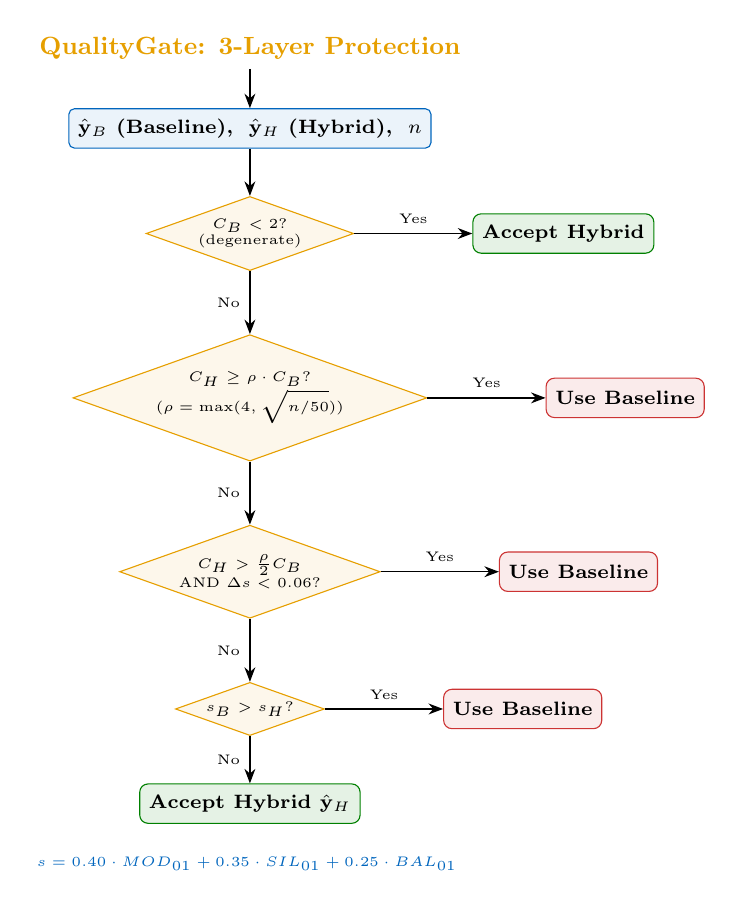
\begin{tikzpicture}[
    >=Stealth, node distance=0.6cm,
    font=\scriptsize,
    input/.style={rectangle, rounded corners=2pt, draw=cb1, fill=cb1!8,
        minimum width=2.5cm, minimum height=0.5cm, align=center,
        font=\scriptsize\bfseries},
    test/.style={diamond, aspect=2.8, draw=cb4, fill=cb4!8,
        minimum width=1.5cm, font=\tiny, align=center, inner sep=1pt},
    accept/.style={rectangle, rounded corners=3pt, draw=cb3, fill=cb3!10,
        minimum width=2cm, minimum height=0.5cm, align=center,
        font=\scriptsize\bfseries},
    reject/.style={rectangle, rounded corners=3pt, draw=cb2, fill=cb2!10,
        minimum width=2cm, minimum height=0.5cm, align=center,
        font=\scriptsize\bfseries},
    arr/.style={-Stealth, line width=0.5pt},
]

% Title
\node[font=\small\bfseries, cb4] (title) {QualityGate: 3-Layer Protection};

% Inputs
\node[input, below=0.5cm of title] (inputs) {$\hat{\mathbf{y}}_B$ (Baseline),\; $\hat{\mathbf{y}}_H$ (Hybrid),\; $n$};

% Layer 0: Degenerate
\node[test, below=0.6cm of inputs] (l0) {$C_B < 2$?\\(degenerate)};
\node[accept, right=1.5cm of l0] (acc0) {Accept Hybrid};

% Layer 1
\node[test, below=0.8cm of l0] (l1) {$C_H \geq \rho \cdot C_B$?\\($\rho = \max(4, \sqrt{n/50})$)};
\node[reject, right=1.5cm of l1] (rej1) {Use Baseline};

% Layer 2
\node[test, below=0.8cm of l1] (l2) {$C_H > \frac{\rho}{2} C_B$\\AND $\Delta s < 0.06$?};
\node[reject, right=1.5cm of l2] (rej2) {Use Baseline};

% Layer 3
\node[test, below=0.8cm of l2] (l3) {$s_B > s_H$?};
\node[reject, right=1.5cm of l3] (rej3) {Use Baseline};

% Final accept
\node[accept, below=0.6cm of l3] (final) {Accept Hybrid $\hat{\mathbf{y}}_H$};

% Arrows
\draw[arr] (title) -- (inputs);
\draw[arr] (inputs) -- (l0);
\draw[arr] (l0) -- node[left, font=\tiny] {No} (l1);
\draw[arr] (l0) -- node[above, font=\tiny] {Yes} (acc0);

\draw[arr] (l1) -- node[left, font=\tiny] {No} (l2);
\draw[arr] (l1) -- node[above, font=\tiny] {Yes} (rej1);

\draw[arr] (l2) -- node[left, font=\tiny] {No} (l3);
\draw[arr] (l2) -- node[above, font=\tiny] {Yes} (rej2);

\draw[arr] (l3) -- node[left, font=\tiny] {No} (final);
\draw[arr] (l3) -- node[above, font=\tiny] {Yes} (rej3);

% Score formula
\node[below=0.3cm of final, font=\tiny\itshape, text=cb1, align=center] {
    $s = 0.40 \cdot \text{MOD}_{01} + 0.35 \cdot \text{SIL}_{01} + 0.25 \cdot \text{BAL}_{01}$
};

\end{tikzpicture}
\end{document}
